\pdfoutput=1
\documentclass[11pt,a4paper]{article}
\usepackage[T1]{fontenc}
\usepackage[utf8]{inputenc}
\usepackage{lmodern}
\usepackage[margin=0.92in]{geometry}
\usepackage{amsmath,amssymb}
\usepackage{booktabs}
\usepackage{graphicx}
\usepackage{microtype}
\usepackage{url}
\usepackage{hyperref}
\usepackage{natbib}
\usepackage{array}
\usepackage{tabularx}
\usepackage{enumitem}
\usepackage{xcolor}

\hypersetup{
  colorlinks=true,
  breaklinks=true,
  linkcolor=blue!65!black,
  citecolor=green!40!black,
  urlcolor=blue!75!black
}
\renewcommand{\topfraction}{0.95}
\renewcommand{\bottomfraction}{0.95}
\renewcommand{\textfraction}{0.05}
\renewcommand{\floatpagefraction}{0.85}
\newcommand{\method}{PromptPrism}

\title{\textbf{Auditing, Pruning, and Stabilizing Compiled Prompts:}\\
\large Coverage-Aware Equivalence Testing and Perturbation Stability Certification for LLMs}
\author{\textbf{Roberto Sanchez}\\PromptPrism Research Group\\\texttt{trev21mx@gmail.com}}
\date{November 24, 2026}

\begin{document}
\setlength{\emergencystretch}{2.5em}
\maketitle

\begin{abstract}
Prompts for Large Language Models (LLMs) often grow long, costly, and fragile as instructions, few-shot examples, and safety rules accumulate by trial and error. Automatic prompt optimizers such as DSPy \texttt{MIPROv2} automate prompt writing, but they typically produce opaque 1,100+ token prompts without proving which pieces actually improve accuracy, whether rare safety rules survive, or whether small formatting changes break performance. We present \method{}~2.1, an open-source statistical auditing framework that tests prompt components in balanced experiments and certifies prompt stability. Compared directly against DSPy \texttt{MIPROv2} on \texttt{gemini-2.5-flash} across three benchmarks (Banking77, SQuAD~2.0, and GSM8K; $N=240$ held-out items), \method{} delivers three practical benefits: (1)~\textbf{safe bloat removal}---auditing compiled DSPy prompts reveals that DSPy's generated instructions are statistically dead weight on Banking77 and SQuAD~2.0, cutting prompt length by 39\%--57\% with matched accuracy and passing stability bounds; (2)~\textbf{rare guardrail protection}---a coverage-aware pruning gate cuts accidental deletion of rare safety rules from 18\%--95\% down to 0\% in calibration and catches 85\% of out-of-scope Banking77 queries where DSPy scores 0\%; and (3)~\textbf{compact, stable standalone prompts}---using structured multi-turn XML framing without DSPy or an expensive proposer model, \method{} matches or edges DSPy on Banking77 (96.3\% vs.\ 95.8\%, $-39\%$ tokens) and GSM8K (95.8\% vs.\ 94.6\%, $-67\%$ tokens), passes strict perturbation stability across all three tasks, and shows why structural scaffolds must stay fixed when pruning redundant pieces.
\end{abstract}

\section{Introduction}
Anyone who builds an application around a Large Language Model (LLM) quickly runs into a familiar problem: prompts grow by accretion. A team starts with a two-sentence instruction, adds a persona, appends a few input--output examples, writes a strict output-format rule, and tacks on a safety guardrail to refuse out-of-scope questions. Months later, the prompt is hundreds or thousands of tokens long, yet nobody can answer three basic engineering questions:
\begin{enumerate}[leftmargin=*,nosep]
    \item \textbf{Attribution:} Which individual pieces of the prompt actually help accuracy, which actively hurt it, and which are dead weight?
    \item \textbf{Safe pruning:} If we delete a seemingly useless sentence to save tokens and latency, how do we make sure we did not accidentally delete a rare safety rule that simply never triggered in our test set?
    \item \textbf{Stability:} If a user changes spacing, delimiters, or minor wording, will the prompt keep working reliably or quietly collapse?
\end{enumerate}

Today's prompting tools split into two camps that leave these questions unanswered. \emph{Evaluation harnesses} score a prompt as a single monolithic blob, reporting an overall accuracy number without revealing which clauses caused a gain or whether a small difference is just random question-sampling noise \citep{miller2024adding,mizrahi2024state}. Conversely, \emph{automatic prompt optimizers} such as APE \citep{zhou2023large}, OPRO \citep{yang2023large}, DSPy \citep{khattab2024dspy}, and \texttt{MIPROv2} \citep{opsahl2024optimizing} search automatically over rewritten instructions and bootstrapped examples to maximize a validation score. While powerful, they frequently emit $1{,}000+$-token composite prompts without checking whether every generated instruction and example earns its token cost, whether rare edge-case guardrails survive, or whether the compiled prompt is resilient to formatting shifts \citep{sclar2024quantifying,habba2025dove}.

\begin{table}[!ht]
\centering
\footnotesize
\setlength{\tabcolsep}{4.5pt}
\caption{At-a-glance comparison of automatic prompt compilation (DSPy \texttt{MIPROv2}) versus statistical prompt auditing (\method{}~2.1). The two paradigms are both direct comparators and natural complements: \method{} can audit and shrink prompts compiled by DSPy, or optimize structured prompts natively without a proposer model.}
\label{tab:p2_comparison}
\begin{tabularx}{\textwidth}{@{}l>{\raggedright\arraybackslash}X>{\raggedright\arraybackslash}X@{}}
\toprule
\textbf{Dimension} & \textbf{DSPy \texttt{MIPROv2} (Prompt Compiler)} & \textbf{\method{}~2.1 (Statistical Auditor)} \\
\midrule
Primary goal & Search for new wording and bootstrapped few-shot demos using a strong proposer LM. & Measure each clause/demo's causal effect, prune provable bloat safely, and certify stability. \\
Prompt transparency & Black-box composite output ($1{,}180+$ tokens typical); no per-clause attribution. & Exact per-component effect ($\hat{\Delta}$), confidence interval, token cost, and pruning verdict. \\
Rare safety guardrails & Optimized on average traffic; missed $0/20$ out-of-scope Banking77 cases. & Coverage gate protects unexercised rules; rescued Banking77 guardrail ($17/20$ pass, $85\%$). \\
Token efficiency & Long prompts and verbose instructions (many components statistically neutral). & Cuts DSPy prompts by $39\%$--$57\%$, or runs standalone at $105$--$717$ tokens ($-39\%$ to $-74\%$). \\
Perturbation stability & Strong on inner-field tweaks due to structured framing, but uncertified by default. & Formal paired perturbation certificate ($U_{95,\mathrm{sim}} < 0.02$) separating genuine drops from noise. \\
\bottomrule
\end{tabularx}
\end{table}

\subsection{Background and Statistical Concepts in Plain Language}
This paper builds on our prior empirical methodology audit of 1,033 retrospective multi-prompt benchmark cubes ($7.0\text{M}$ outcomes) and $501{,}300$ prospective LLM calls, which established three baseline facts: (i)~structured orthogonal screens match random and Bayesian search on peak accuracy while cutting 6-factor effect-estimation error by $35.38\%$; (ii)~$79\%$--$85\%$ of apparent higher-order interaction variance on single-task benchmarks is simply item-sampling noise; and (iii)~contrast-specific item-clustered $t$-tests control false discoveries at $4.0\%$--$5.1\%$, whereas pooled fixed-block ANOVA inflates false positives to $18.4\%$.

Because statistical terminology from experimental design can look dense at first glance, four core tools used throughout this paper are summarized intuitively below:
\begin{itemize}[leftmargin=*,nosep]
    \item \textbf{Fractional factorial screening ($2^{k-p}$):} Suppose a prompt has $k=6$ toggleable components (ON/OFF). Testing every combination takes $2^6=64$ runs. A balanced \emph{Resolution-IV} fraction ($2^{6-2}_{\mathrm{IV}}$) runs only 16 carefully chosen combinations where each component is ON 8 times and OFF 8 times, allowing us to estimate every component's main effect accurately at one-quarter the cost \citep{box2005statistics,wu2011experiments}.
    \item \textbf{Paired item-clustered $t$-tests and BH control:} Because every prompt variant is evaluated on the \emph{exact same} test questions, we compute the ON-minus-OFF score difference on each question first. Pairing cancels out question difficulty (easy vs.\ hard items), shrinking variance sharply \citep{miller2024adding}. We then adjust $p$-values with Benjamini--Hochberg (BH) \citep{benjamini1995controlling} so testing multiple prompt clauses at once does not inflate false discoveries.
    \item \textbf{Equivalence testing (TOST):} A textbook significance test only asks ``is this clause different from zero?'' Failing to reach $p < 0.05$ does \emph{not} prove a clause is useless---the sample might simply be too small. Two One-Sided Tests (TOST) \citep{schuirmann1987comparison} reverses the question: it tests whether a clause's true impact is provably trapped inside a tiny equivalence band $[-m_F, +m_F]$ (e.g., $\pm 2$ percentage points), certifying that deleting it is safe.
    \item \textbf{Simultaneous stability certificate ($U_{95,\mathrm{sim}} < \epsilon$):} Rather than checking only clean accuracy, we test a locked prompt across five minor perturbations (an identical repeat, extra whitespace, delimiter changes, and two paraphrases). Using paired bootstrap resampling across all five environments at once, we compute a 95\% upper bound $U_{95,\mathrm{sim}}$ on the worst accuracy drop; the prompt earns \texttt{PASS} only if we are 95\% confident its worst drop is under $\epsilon = 0.02$ ($2\text{ pp}$).
\end{itemize}

\subsection{Contributions}
Applying these statistical tools to real production prompts exposes three unsolved practical hazards: (1)~baseline-only TOST accidentally deletes rare safety guardrails that never fired during routine traffic; (2)~compiled DSPy prompts contain substantial redundant bloat; and (3)~flat prompts frequently fail strict stability bounds, while blindly deleting every individually neutral piece at once can strip all structural anchors simultaneously. \method{}~2.1\footnote{Open-source code, 310 automated tests, and all benchmark JSON summaries are available at \url{https://github.com/robsanmx/prompt_prism}.} addresses all three gaps with:
\begin{enumerate}[leftmargin=*,nosep]
    \item \textbf{Coverage-aware clause pruning and frozen synthetic test sets} (Section~\ref{sec:coverage_gate}), pairing baseline TOST with targeted non-inferiority over blind-tagged, SHA-256-frozen edge-case checks.
    \item \textbf{Stability-aware clause attribution, structured multi-turn XML framing, and diagnostic perturbation certificates} (Section~\ref{sec:stability_upgrades}), preventing pruning of \texttt{STABILIZING} clauses and distinguishing genuine perturbation drops from underpowered sample sizes.
    \item \textbf{End-to-end empirical evaluation} (Section~\ref{sec:results}) spanning Monte Carlo calibration, a live two-task synthetic test-set pilot, a three-task head-to-head and post-compilation bloat audit of DSPy \texttt{MIPROv2}, and a three-task \method{}-native stability upgrade study with zero DSPy calls---including an explicit empirical demonstration and fix for the \emph{simultaneous multi-factor pruning hazard}.
\end{enumerate}

\section{Related Work}
\paragraph{Prompt Sensitivity and Statistical LLM Evaluation.}
Small changes in prompt delimiters, spacing, or phrasing can shift LLM accuracy by double-digit percentages \citep{sclar2024quantifying,mizrahi2024state,habba2025dove,habba2025promptsuite}. Recent statistical evaluation literature emphasizes paired item-level standard errors \citep{miller2024adding} and query-efficient multi-prompt estimation via item-response theory \citep{polo2024efficient,polo2024tinybenchmarks}. Our work extends paired item-clustered inference from passive error bars to actionable \emph{clause-pruning verdicts} via TOST equivalence \citep{schuirmann1987comparison}, BH false-discovery control \citep{benjamini1995controlling}, and fail-closed simultaneous perturbation envelopes.

\paragraph{Automatic Prompt Optimization and Factorial Design.}
Black-box prompt optimizers---including APE \citep{zhou2023large}, OPRO \citep{yang2023large}, bandit-based best-arm identification \citep{shi2024efficient}, combinatorial Bayesian optimization \citep{baptista2018bayesian}, and DSPy/\texttt{MIPROv2} \citep{khattab2024dspy,opsahl2024optimizing}---excel at searching candidate instructions and bootstrapped few-shot demonstrations. Classical Design of Experiments (DoE) \citep{plackett1946design,box2005statistics,wu2011experiments,montgomery2017design} instead focuses on orthogonal attribution of modular factors. Rather than treating these approaches as mutually exclusive, we show how compiled optimizer artifacts can be decomposed into binary factors, audited orthogonally, pruned safely, and certified under explicit perturbation envelopes---and how structured native scaffolds can match or outperform compiled prompts at a fraction of the token cost.

\section{Coverage-Aware Clause Pruning and Frozen Synthetic Test Generation}
\label{sec:coverage_gate}

\subsection{Why Naive Pruning Deletes Important Safety Rules}
Consider a simple thought experiment. Suppose your banking chatbot prompt includes a safety rule: \emph{``If the user asks something outside the allowed banking intents, reply \texttt{OUT\_OF\_SCOPE}.''} Now suppose your evaluation dataset contains 120 normal customer queries, and \emph{zero} of them are out-of-scope. When you test the prompt with the safety rule ON versus OFF, the scores look identical---not because the rule is useless, but because nothing in the test set ever triggered it.

This is not hypothetical. Auditing full 64-run cubes ($N = 120$ screen items, \texttt{gemini-2.5-flash}) under baseline-only TOST ($m_F = 0.02$) marked \texttt{grounding\_\allowbreak guardrail} (Factor~$E$) as \texttt{SAFE\_TO\_PRUNE} on both \texttt{banking77\_\allowbreak intent} ($\hat{\Delta} = -0.76\text{ pp}$, $\mathrm{SE}=0.49\text{ pp}$, $\mathrm{TOST}\ p = 0.0059$) and \texttt{squad2\_\allowbreak grounded\_qa} ($\hat{\Delta} = -0.29\text{ pp}$, $\mathrm{SE}=0.33\text{ pp}$, $\mathrm{TOST}\ p = 5.5\times 10^{-7}$). Inspecting the locked datasets revealed why: $0/680$ Banking77 items were out-of-scope and $0/680$ SQuAD~2.0 items were unanswerable. Baseline equivalence mistook \emph{zero test coverage} for \emph{proof of dead prompt bloat}.

\subsection{Dual-Estimand Coverage Gate (Schema v2.1.0)}
To prevent this failure mode, \method{} evaluates each binary clause $j$ on two separate paired item-clustered estimands whenever a per-clause coverage map $T_j \subseteq \{1,\dots,N\}$ (linking clauses to the edge cases that exercise them) is supplied:
\begin{enumerate}[leftmargin=*,nosep]
    \item \textbf{Baseline traffic estimand ($F$):} Paired item-clustered contrast $\hat{\Delta}_{F,j}$, BH-adjusted $q_{F,j}$ across all $k$ factors, and two-sided TOST equivalence $p_{\mathrm{TOST},j}$ against margin $m_F$ computed strictly on normal baseline items $F$, so oversampled edge cases never distort average-traffic estimates.
    \item \textbf{Targeted coverage estimand ($T_j$):} Paired item-clustered contrast $\hat{\Delta}_{T,j}$, separate BH-adjusted $q_{T,j}$ across covered factors ($n_{T,j} \ge 2$), and a one-sided targeted non-inferiority test of removing the clause:
    \[
        H_0:\; s\Delta_{T,j} \ge m_T \qquad \text{vs.} \qquad H_1:\; s\Delta_{T,j} < m_T,
    \]
    where $s = +1$ when higher scores are better ($-1$ for error minimization), with calibrated default targeted margin $m_T = \max(2m_F, 0.08)$ and minimum paired coverage $n_{\min} = 20$.
\end{enumerate}

A clause earns \texttt{SAFE\_TO\_PRUNE} \emph{only} when it passes all three checks: (i)~neutral on normal traffic ($p_{\mathrm{TOST},j} < \alpha$), (ii)~adequately exercised on targeted cases ($n_{T,j} \ge n_{\min}$), and (iii)~removing it is provably non-inferior on those targeted cases ($p_{\mathrm{NI},T,j} < \alpha$). Otherwise, \method{} assigns one of seven fail-safe verdicts in priority order (Table~\ref{tab:p2_verdicts}).

\begin{table}[!ht]
\centering
\footnotesize
\setlength{\tabcolsep}{4.0pt}
\caption{Fail-safe seven-verdict priority hierarchy in \method{}~2.1 (schema v2.1.0). A clause is never deleted unless both normal traffic and targeted edge cases confirm it is unneeded.}
\label{tab:p2_verdicts}
\begin{tabularx}{\textwidth}{@{}ll>{\raggedright\arraybackslash}X@{}}
\toprule
\textbf{Priority} & \textbf{Verdict} & \textbf{Plain-English Meaning \& Recommended Action} \\
\midrule
1 & \texttt{CONFLICT\_REVIEW} & Baseline and targeted effects pull in opposite directions, or the clause hurts baseline traffic without enough targeted items ($n_{T,j} < n_{\min}$) to rule out edge-case benefit. Inspect manually. \\
2 & \texttt{KEEP} & Statistically helpful on normal baseline traffic ($q_{F,j} < \alpha$, $s\hat{\Delta}_{F,j} > 0$). Keep in prompt. \\
3 & \texttt{REMOVE\_HARMFUL} & Statistically harmful on baseline traffic ($q_{F,j} < \alpha$, $s\hat{\Delta}_{F,j} < 0$) and safely covered on targeted items ($n_{T,j} \ge n_{\min}$ without targeted benefit). Remove to improve accuracy. \\
4 & \texttt{UNTESTED} & Zero targeted test items exercise this clause ($n_{T,j} = 0$). Do \emph{not} delete blindly; add targeted checks first. \\
5 & \texttt{KEEP\_TARGETED} & Neutral on normal traffic, but statistically helpful on targeted edge cases ($n_{T,j} \ge n_{\min}$, $q_{T,j} < \alpha$, $s\hat{\Delta}_{T,j} > 0$). Keep to protect edge-case behavior. \\
6 & \texttt{SAFE\_TO\_PRUNE} & Passes baseline TOST ($p_{\mathrm{TOST},j} < \alpha$), coverage ($n_{T,j} \ge n_{\min}$), and targeted non-inferiority ($p_{\mathrm{NI},T,j} < \alpha$). Provably safe to delete individually. \\
7 & \texttt{INCONCLUSIVE\_NEED\_MORE\_ITEMS} & Neither clearly helpful/harmful nor tightly bounded inside the equivalence margin yet. Collect more paired items before deciding. \\
\bottomrule
\end{tabularx}
\end{table}

\subsection{Frozen, Blind-Tagged Synthetic Test Generation}
When teams lack hand-labelled edge-case suites, \method{} provides \texttt{TestSetGenerator} and \texttt{CheckSuiteMetric} with four built-in methodological safeguards:
\begin{enumerate}[leftmargin=*,nosep]
    \item \textbf{Clause-role honesty:} Targeted behavioral checks are generated only for \texttt{conditional\_rule} clauses (such as refusal guardrails or output-format constraints). \texttt{global\_scaffold} clauses (personas, chain-of-thought hints, few-shot demos, self-verification) are scored strictly on normal task correctness so a harmful scaffold cannot game a tautological surface check.
    \item \textbf{Deterministic checks first:} Checks prefer exact, regex, substring, or JSON-schema validators filtered by $(\texttt{reference\_pass}, \texttt{reference\_fail})$ passability/failability tests, raw-input-echo rejection, ReDoS regex guards, and near-duplicate Jaccard deduplication ($0.9$).
    \item \textbf{Independent blind coverage tagging:} A separate tagger assigns which clauses each synthetic item exercises \emph{without} seeing the generator's \texttt{intended\_factor} label, requiring agreement by default to prevent self-fulfilling tags.
    \item \textbf{Cryptographic freeze and honest tiering:} Generated suites are split into stratified \texttt{discovery} and \texttt{confirmation} partitions, frozen under canonical-JSON SHA-256 hashes, and stamped \texttt{evidence\_tier = "predicted (synthetic tests)"} until verified on real traffic.
\end{enumerate}

\section{Stability-Aware Attribution and Perturbation Certification}
\label{sec:stability_upgrades}

\subsection{Structured Multi-Turn Framing and Toggleable Demo Factors}
Flat single-user prompts that glue sections together with plain-text brackets (e.g., \texttt{[EXAMPLES]}, \texttt{[TASK INPUT]}) frequently degrade when outer delimiters or whitespace shift. \method{}~2.1 introduces two clean building blocks:
\begin{itemize}[leftmargin=*,nosep]
    \item \textbf{\texttt{PromptTemplate.\allowbreak structured\_chat}:} \texttt{PromptComposer.\allowbreak compose\_messages()} merges only \emph{consecutive} same-role sections, preserving true alternating \texttt{user}/\texttt{assistant} demonstration turns and explicit XML (\texttt{<query>...</query>}) or bracket (\texttt{[[ \#\# query \#\# ]]}) field tags.
    \item \textbf{\texttt{Factor.demo} and \texttt{FactorSet.\allowbreak from\_\allowbreak candidate\_demos}:} Candidate in-domain demonstrations---either error-mined strictly from the \texttt{screen} split or extracted from a compiled DSPy program---become toggleable binary factors. This lets TOST keep only the examples that genuinely earn their token cost.
\end{itemize}

\subsection{Stability-Aware Clause Attribution (\texttt{env\_col} / \texttt{ref\_env})}
A prompt clause might look neutral on clean inputs yet quietly protect accuracy when inputs are paraphrased or reformatted. When screening spans a clean reference environment (\texttt{ref\_env}) plus semantic-preserving perturbations, \texttt{diagnose(..., env\_col="env\_id", ref\_env="ref")} estimates clean main effects on \texttt{ref\_env} and separately computes each item's paired perturbation drop:
\[
    d_{i,r} = s \cdot \bigl(y_{i,r,\mathrm{ref}} - \bar{y}_{i,r,\mathrm{pert}}\bigr).
\]
It then runs a separate BH-corrected item-clustered $t$-test on the drop contrast $\Delta_{\mathrm{drop},j} = \bar{d}_{j=1} - \bar{d}_{j=0}$. Clauses that significantly shrink the drop ($q_{\mathrm{drop},j} < \alpha$ and $\Delta_{\mathrm{drop},j} < 0$) are tagged \texttt{STABILIZING} and shielded from deletion (a clean-neutral stabilizing clause promotes to \texttt{KEEP}; a clean-harmful stabilizing clause routes to \texttt{CONFLICT\_REVIEW}). Clauses that worsen drops ($q_{\mathrm{drop},j} < \alpha$ and $\Delta_{\mathrm{drop},j} > 0$) are flagged \texttt{FRAGILE}.

\subsection{Precision-vs.-Genuine Stability Certificate Diagnostics}
Given paired item scores across clean reference \texttt{ref} and perturbation environments $\mathcal{E}$, \texttt{evaluate\_\allowbreak simultaneous\_\allowbreak perturbation\_\allowbreak certificate()} computes a paired cluster-bootstrap simultaneous 95\% upper bound $U_{95,\mathrm{sim}}$ on the maximum environment drop $\hat{d}_{\max} = \max_{e \in \mathcal{E}}(\bar{y}_{\mathrm{ref}} - \bar{y}_e)$, issuing \texttt{PASS} iff $U_{95,\mathrm{sim}} < \epsilon$ (default $\epsilon = 0.02$) and hashing the pinned \texttt{OperatingEnvelopeSpec}.

Importantly, a certificate can fail for two very different reasons: either the prompt genuinely breaks ($\hat{d}_{\max} \ge \epsilon$), or the drop is tiny ($\hat{d}_{\max} < \epsilon$) but $N=240$ items is too small to shrink the 95\% confidence bound below $0.02$. \method{}~2.1 automatically reports \texttt{worst\_env\_id}, per-environment drops and standard errors, the repeat-pass noise floor (\texttt{repeat\_noise\_se}), and an actionable \texttt{diagnostic\_note} separating \emph{genuine perturbation drops} from \emph{precision-limited failures} along with an estimated minimum sample size \texttt{recommended\_min\_n}.

\section{Empirical Evaluation}
\label{sec:results}
All live experiments use pinned \texttt{gemini-2.5-flash} (\texttt{temperature=0.0}, \texttt{thinkingBudget=0}, \texttt{max\_output\_tokens=512}) on untouched splits (\texttt{screen} $N=120$, \texttt{validation} $N=60$, \texttt{clean\_confirmation} $N=240$) and five paired perturbation environments (\texttt{repeat\_r2}, \texttt{fmt\_whitespace}, \texttt{fmt\_delimiter}, \texttt{word\_paraphrase\_1}, \texttt{word\_paraphrase\_2}).

\subsection{Monte Carlo Calibration of Coverage-Gated Pruning}
Across 16-run $2^{6-2}_{\mathrm{IV}}$ designs ($N_{\mathrm{base}}=100$, $m_F=0.03$, $n_{\min}=20$, $\alpha=0.05$, 100 replications/cell, realistic paired contrast SDs $\sigma_c \in \{0.08, 0.11, 0.15\}$), Table~\ref{tab:p2_mc} shows that unguarded baseline TOST falsely deletes real conditional rules ($\tau_T \in \{0.15, 0.25\}$) in \textbf{22\%--95\%} of runs when the rule triggers on $p=2\%$ of traffic, and \textbf{18\%--78\%} at $p=5\%$. Adding the coverage gate ($n_T=35, m_T=0.08$) drives false deletions to \textbf{0.0\%} across all 24 cells while sustaining \textbf{100\% / 100\% / 94\%} targeted non-inferiority pruning power on truly dead clauses.

\begin{table}[!ht]
\centering
\scriptsize
\setlength{\tabcolsep}{2.8pt}
\caption{Monte Carlo calibration of the coverage-aware pruning gate (16-run $2^{6-2}_{\mathrm{IV}}$, $N_{\mathrm{base}}=100$, $m_F=0.03$, $n_{\min}=20$, $\alpha=0.05$, 100 replicates/cell). Part~A: false-prune rate on a real conditional rule ($\tau_T = 0.15$ / $0.25$, $n_T = 35, m_T = 0.08$). Part~B: targeted non-inferiority (NI) and joint \texttt{SAFE\_TO\_PRUNE} power on a true dead clause ($\tau_F = \tau_T = 0$).}
\label{tab:p2_mc}
\begin{tabularx}{\textwidth}{@{}llrrrr>{\raggedright\arraybackslash}X@{}}
\toprule
\multicolumn{7}{@{}l}{\textit{Part A: Real Conditional Rule False-Prune Rate ($\tau_T = 0.15$ / $0.25$, $n_T=35$, $m_T=0.08$)}} \\
\textbf{$\sigma_c$} & \textbf{Trigger $p$} & \textbf{FP No Gate} & \textbf{FP Gated} & \textbf{Keep Gated} & \textbf{Reps} & \textbf{Interpretation} \\
\midrule
$0.08$ & $0.02$ / $0.05$ & $95\%$--$91\%$ / $78\%$--$52\%$ & \textbf{0.0\%} & $99\%$--$100\%$ & 100 & High baseline TOST power amplifies false prunes \\
$0.11$ & $0.02$ / $0.05$ & $65\%$--$61\%$ / $62\%$--$39\%$ & \textbf{0.0\%} & $100\%$ & 100 & Gate eliminates rare-rule deletion \\
$0.15$ & $0.02$ / $0.05$ & $22\%$--$23\%$ / $21\%$--$18\%$ & \textbf{0.0\%} & $99\%$ & 100 & Gate retains rule even at high contrast SD \\
$0.08$--$0.15$ & $0.20$ / $1.00$ & $0\%$--$5\%$ / $0.0\%$ & \textbf{0.0\%} & $100\%$ & 100 & Frequent rules already visible on baseline \\
\midrule
\multicolumn{7}{@{}l}{\textit{Part B: True Dead-Clause Pruning Power ($\tau_F = \tau_T = 0$, Real-Rule FP $= 0.0\%$ Across All Rows)}} \\
\textbf{$\sigma_c$} & \textbf{$n_T$} & \textbf{NI ($0.05$)} & \textbf{NI ($0.06$)} & \textbf{NI ($0.08$)} & \textbf{Joint ($0.08$)} & \textbf{Calibration Decision} \\
\midrule
$0.08$ & $20$ / $35$ & $98\%$ / $100\%$ & $100\%$ / $100\%$ & \textbf{100\% / 100\%} & $92\%$ / $91\%$ & Full power across all margins \\
$0.11$ & $20$ / $35$ & $76\%$ / $83\%$ & $88\%$ / $95\%$ & \textbf{96\% / 100\%} & $73\%$ / $71\%$ & $m_T{=}0.08$ clears $95\%$ NI target \\
$0.15$ & $20$ / $35$ & $47\%$ / $59\%$ & $61\%$ / $74\%$ & \textbf{84\% / 94\%} & $24\%$ / $24\%$ & Default: $m_T{=}\max(2m_F, 0.08)$ \\
\bottomrule
\end{tabularx}
\end{table}

\subsection{Live Two-Task Synthetic Test-Set Pilot}
Generating frozen deterministic test suites with \texttt{gemini-2.5-pro} (temperature $0.7$ generator, temperature $0.0$ independent blind tagger, $0\%$ LLM-judge fallback) and evaluating 16-run $2^{6-2}_{\mathrm{IV}}$ screens on \texttt{gemini-2.5-flash} yields $0/12$ dangerous prune flips across \texttt{banking77\_intent} ($470/470$ cases) and \texttt{squad2\_grounded\_qa} ($357/470$ cases; Table~\ref{tab:p2_testgen}). Both unexercised \texttt{grounding\_guardrail} clauses flip from Real-v4's false \texttt{SAFE\_TO\_PRUNE} to \texttt{KEEP\_TARGETED} ($+75.71\text{ pp}$, $q_T = 1.6\times 10^{-12}$ on Banking77; $+2.23\text{ pp}$, $q_T = 0.0048$ on SQuAD~2.0), and clause-role separation prevents harmful \texttt{brief\_reasoning} from flipping to \texttt{KEEP}. The pilot also surfaces two real operational boundaries: long-context anchored-regex baseline shortfalls on SQuAD~2.0 ($N_F = 19$, flagged by the automatic small-$N$ warning) and a $B \times D$ confirmation interaction ($0.793 \to 0.750$) illustrating why synthetic audits carry \texttt{evidence\_tier = "predicted (synthetic tests)"} until confirmed on real items.

\begin{table*}[!ht]
\centering
\scriptsize
\setlength{\tabcolsep}{3.0pt}
\caption{Live two-task synthetic test-generation pilot (\texttt{gemini-2.5-pro} $\to$ \texttt{gemini-2.5-flash}, 16-run $2^{6-2}_{\mathrm{IV}}$, $m_F=0.02, m_T=0.08, n_{\min}=20$, $0\%$ LLM judge) vs.\ full 64-run Real-v4 reference audits ($N=120$, $0$ out-of-scope/unanswerable items). Abbreviations: \texttt{REM}=\texttt{REMOVE\_\allowbreak HARMFUL}, \texttt{PRUNE}=\texttt{SAFE\_\allowbreak TO\_\allowbreak PRUNE}, \texttt{KEEP\_T}=\texttt{KEEP\_\allowbreak TARGETED}, \texttt{INC}=\texttt{INCONCLUSIVE\_\allowbreak NEED\_\allowbreak MORE\_\allowbreak ITEMS}, \texttt{UNT}=\texttt{UNTESTED}.}
\label{tab:p2_testgen}
\begin{tabular}{@{}llrrlrrrrl@{}}
\toprule
\textbf{Role} & \textbf{Clause (Factor)} & \multicolumn{3}{c}{\textbf{Real-v4 64-Run ($N{=}120$)}} & \multicolumn{5}{c}{\textbf{Live Synthetic 16-Run ($2^{6-2}_{\mathrm{IV}}$)}} \\
\cmidrule(lr){3-5}\cmidrule(lr){6-10}
 & & \textbf{$\hat{\Delta}_{\mathrm{real}}$} & \textbf{TOST $p$} & \textbf{Verdict} & \textbf{$\hat{\Delta}_F$} & \textbf{TOST $p$} & \textbf{$n_T$} & \textbf{$\hat{\Delta}_T$} & \textbf{Verdict} \\
\midrule
\multicolumn{10}{@{}l}{\textit{Banking77 Intent ($470/470$ cases; $N_F{=}100$ baseline; confirmation $0.900 \to 0.900$, $0.00\text{ pp}$)}} \\
\texttt{cond\_rule} & \texttt{grounding\_guardrail} (E) & $-0.76\text{ pp}$ & $0.0059$ & \texttt{PRUNE} & $-0.50\text{ pp}$ & $0.037$ & $35$ & \textbf{$+75.71\text{ pp}$} & \textbf{\texttt{KEEP\_T}} \\
\texttt{cond\_rule} & \texttt{strict\_output\_contract} (D) & $+1.80\text{ pp}$ & $0.350$ & \texttt{KEEP} & $-0.25\text{ pp}$ & $<10^{-4}$ & $39$ & \textbf{$+12.18\text{ pp}$} & \textbf{\texttt{KEEP\_T}} \\
\texttt{scaffold} & \texttt{few\_shot\_demos} (C) & $+1.85\text{ pp}$ & $0.446$ & \texttt{INC} & $+1.75\text{ pp}$ & $0.349$ & $23$ & $+5.98\text{ pp}$ & \texttt{KEEP} \\
\texttt{scaffold} & \texttt{brief\_reasoning} (B) & $-3.88\text{ pp}$ & $0.988$ & \texttt{REM} & $-0.25\text{ pp}$ & $0.019$ & $3$ & $+0.00\text{ pp}$ & \texttt{INC} \\
\texttt{scaffold} & \texttt{self\_verification} (F) & $+0.91\text{ pp}$ & $0.0017$ & \texttt{KEEP} & $-0.25\text{ pp}$ & $<10^{-4}$ & $0$ & --- & \texttt{UNT} \\
\texttt{scaffold} & \texttt{specialist\_persona} (A) & $+0.86\text{ pp}$ & $0.0037$ & \texttt{PRUNE} & $-0.50\text{ pp}$ & $0.0004$ & $4$ & $+6.25\text{ pp}$ & \texttt{INC} \\
\midrule
\multicolumn{10}{@{}l}{\textit{SQuAD 2.0 QA ($357/470$ cases; $N_F{=}19$ shortfall [warned]; confirmation $0.793 \to 0.750$, $-4.30\text{ pp}$)}} \\
\texttt{cond\_rule} & \texttt{grounding\_guardrail} (E) & $-0.29\text{ pp}$ & $<10^{-6}$ & \texttt{PRUNE} & $+1.97\text{ pp}$ & $0.495$ & $129$ & \textbf{$+2.23\text{ pp}$} & \textbf{\texttt{KEEP\_T}} \\
\texttt{cond\_rule} & \texttt{strict\_output\_contract} (D) & $+8.83\text{ pp}$ & $1.000$ & \texttt{KEEP} & $+5.26\text{ pp}$ & $0.889$ & $153$ & \textbf{$+11.52\text{ pp}$} & \textbf{\texttt{KEEP\_T}} \\
\texttt{scaffold} & \texttt{few\_shot\_demos} (C) & $+13.74\text{ pp}$ & $1.000$ & \texttt{KEEP} & $+8.55\text{ pp}$ & $0.968$ & $153$ & $+13.48\text{ pp}$ & \texttt{KEEP} \\
\texttt{scaffold} & \texttt{brief\_reasoning} (B) & $-10.12\text{ pp}$ & $1.000$ & \texttt{REM} & $-11.84\text{ pp}$ & $0.990$ & $41$ & $-7.93\text{ pp}$ & \textbf{\texttt{REM}} \\
\texttt{scaffold} & \texttt{specialist\_persona} (A) & $+1.36\text{ pp}$ & $0.056$ & \texttt{KEEP} & $+1.32\text{ pp}$ & $0.375$ & $10$ & $+5.00\text{ pp}$ & \texttt{INC} \\
\texttt{scaffold} & \texttt{self\_verification} (F) & $-0.78\text{ pp}$ & $0.0033$ & \texttt{PRUNE} & $+9.87\text{ pp}$ & $0.978$ & $0$ & --- & \texttt{KEEP} \\
\bottomrule
\end{tabular}
\end{table*}

\subsection{DSPy \texttt{MIPROv2} Benchmark and Post-Compilation Bloat Audit (Tracks A \& B)}
To compare \method{} directly against a widely used prompt optimizer, we compiled \texttt{dspy.MIPROv2} (\texttt{dspy==3.5.0}; \texttt{gemini-2.5-pro} proposer with \texttt{reasoning\_effort="low"}, 7~candidates, 20~trials, up to 4~bootstrapped and 4~labeled demos; task LM \texttt{gemini-2.5-flash} with \texttt{reasoning\_effort="off"}) strictly on the \texttt{screen} ($N=120$) and \texttt{validation} ($N=60$) splits, then evaluated both the compiled DSPy program and the Real-v4 flat \method{} winner on untouched $N=240$ confirmation items across all six environments (Track~A). Next, in Track~B, we unpacked each multi-component DSPy prompt into binary \method{} factors (\texttt{dspy\_instruction} + \texttt{dspy\_demo\_1..4}), ran a 16-run $2^{5-1}_{\mathrm{V}}$ TOST screen on \texttt{screen} ($N=120$, $m_F=0.02$), deleted every \texttt{SAFE\_TO\_PRUNE} piece, and re-certified on \texttt{clean\_confirmation} ($N=240$). Figure~\ref{fig:p2_dspy} and Table~\ref{tab:p2_dspy} summarize the findings.

\begin{figure*}[!ht]
\centering
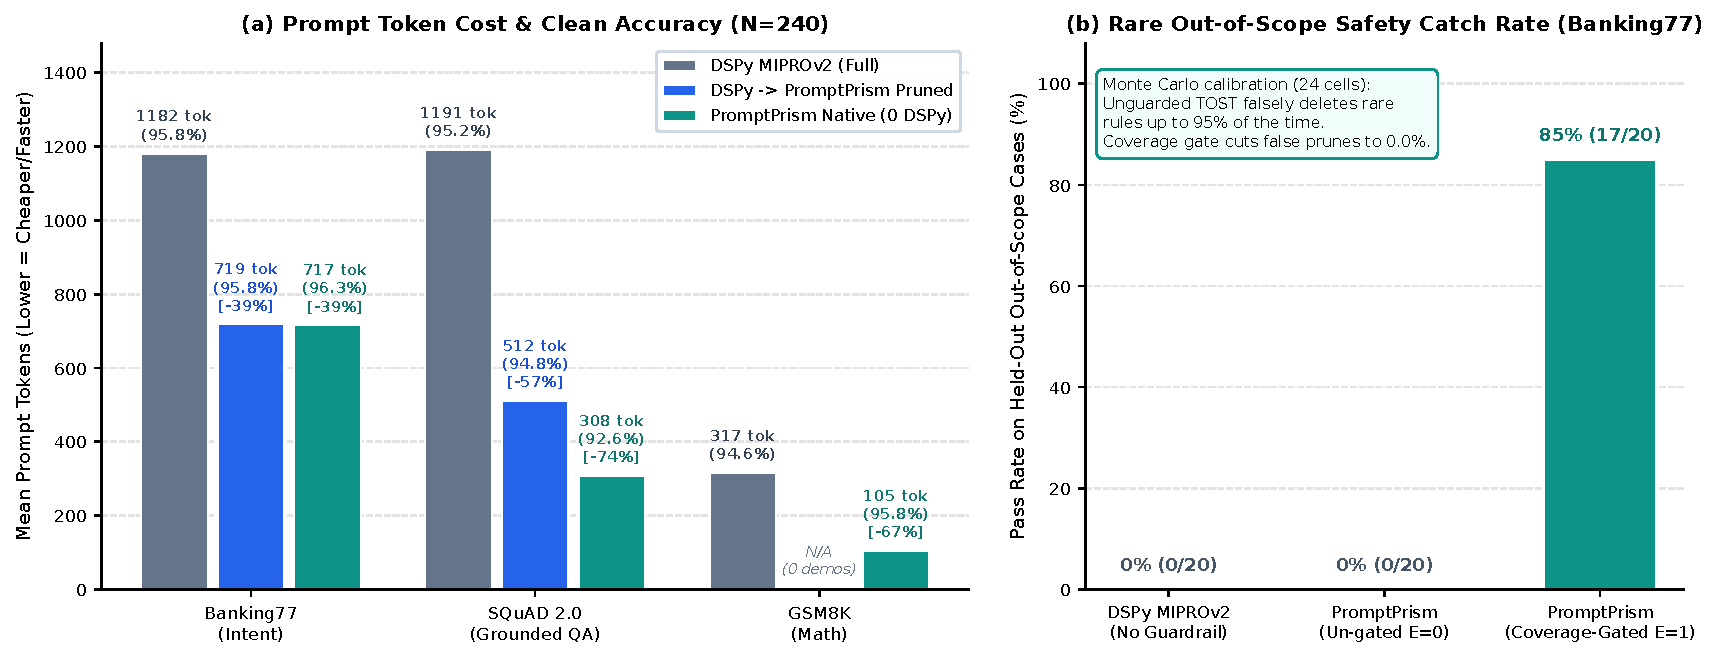
\includegraphics[width=\textwidth]{fig_p2_dspy_comparison.pdf}
\caption{Visual comparison of DSPy \texttt{MIPROv2} vs.\ \method{}~2.1 on \texttt{gemini-2.5-flash} ($N=240$ untouched confirmation items). \textbf{(a)}~Prompt token cost and clean accuracy: auditing DSPy with \method{} cuts $39\%$--$57\%$ of prompt tokens at matched accuracy, while standalone \method{} Native (zero DSPy, zero Pro proposer) matches or edges DSPy on Banking77 and GSM8K at $39\%$--$67\%$ fewer prompt tokens. \textbf{(b)}~Held-out Banking77 out-of-scope safety audit ($N=20$): both DSPy \texttt{MIPROv2} and un-gated \method{} score $0\%$, whereas \method{}'s coverage-gated guardrail rescues $85\%$ ($17/20$).}
\label{fig:p2_dspy}
\end{figure*}

\begin{table*}[!ht]
\centering
\scriptsize
\setlength{\tabcolsep}{2.6pt}
\caption{Track~A (head-to-head) and Track~B (DSPy $\to$ \method{} TOST pruning) on untouched $N=240$ confirmation items (\texttt{gemini-2.5-flash}, \texttt{temperature=0.0}, \texttt{thinkingBudget=0}). Paired $p$-values compare clean (\texttt{ref}) scores via item/group-clustered $t$-tests. Edge-case pass rates measure $N=20$ held-out frozen confirmation guardrail cases (Banking77 out-of-scope; SQuAD~2.0 unanswerable).}
\label{tab:p2_dspy}
\resizebox{\textwidth}{!}{%
\begin{tabular}{@{}llrrrrrr@{}}
\toprule
\textbf{Task} & \textbf{System} & \textbf{Clean (\texttt{ref})} & \textbf{Max Drop} & \textbf{$U_{95,\mathrm{sim}}$} & \textbf{Cert} & \textbf{Prompt / Out Tok} & \textbf{Edge-Case Pass} \\
\midrule
\texttt{banking77} & Real-v4 Flat \method{} ($E{=}0$) & $95.42\%$ & $2.92\text{ pp}$ & $0.0542$ & \texttt{FAIL} & $290$ / $9.5$ & $0.0\%$ ($85.0\%$ w/ $E{=}1$) \\
 & DSPy \texttt{MIPROv2} Full & $95.83\%$ & $0.42\text{ pp}$ & $0.0195$ & \texttt{PASS} & $1{,}182$ / $17.7$ & $0.0\%$ \\
 & \textbf{DSPy $\to$ \method{} Pruned} ($-3/5$) & \textbf{$95.83\%$} & \textbf{$0.00\text{ pp}$} & \textbf{$0.0083$} & \textbf{\texttt{PASS}} & \textbf{$719$ ($-39.2\%$)} / $17.7$ & --- \\
\midrule
\texttt{squad2} & Real-v4 Flat \method{} ($E{=}0$) & $92.24\%$ & $0.62\text{ pp}$ & $0.0222$ & \texttt{FAIL} & $312$ / $10.3$ & $80.0\%$ ($85.0\%$ w/ $E{=}1$) \\
 & DSPy \texttt{MIPROv2} Full & $95.25\%$ & $0.05\text{ pp}$ & $0.0045$ & \texttt{PASS} & $1{,}191$ / $17.5$ & $95.0\%$ \\
 & \textbf{DSPy $\to$ \method{} Pruned} ($-4/5$) & \textbf{$94.77\%$} & \textbf{$0.39\text{ pp}$} & \textbf{$0.0116$} & \textbf{\texttt{PASS}} & \textbf{$512$ ($-57.0\%$)} / $17.8$ & --- \\
\midrule
\texttt{gsm8k} & Real-v4 Flat \method{} & $95.83\%$ & $0.83\text{ pp}$ & $0.0358$ & \texttt{FAIL} & $146$ / $152.3$ & --- \\
 & DSPy \texttt{MIPROv2} Full ($0$ demos) & $94.58\%$ & $0.42\text{ pp}$ & $0.0193$ & \texttt{PASS} & $317$ / $224.8$ & --- \\
\bottomrule
\end{tabular}}
\end{table*}

Three practical takeaways stand out from Figure~\ref{fig:p2_dspy} and Table~\ref{tab:p2_dspy}:
\begin{enumerate}[leftmargin=*,nosep]
    \item \textbf{Compiled DSPy prompts hide substantial dead weight:} On \texttt{banking77}, 3 of 5 compiled pieces---including DSPy's 98-token generated instruction ($\hat{\Delta} = -0.31\text{ pp}$, $\mathrm{TOST}\ p = 2.1\times 10^{-11}$), \texttt{demo\_2} ($184$ tok), and \texttt{demo\_4} ($181$ tok)---proved \texttt{SAFE\_TO\_PRUNE}. Deleting them saved \textbf{$-463$ prompt tokens ($-39.2\%$)}, kept exact \textbf{$95.83\%$} accuracy ($0.00\text{ pp}$, $p = 1.0$), and more than halved $U_{95,\mathrm{sim}}$ ($0.0195 \to 0.0083$). On \texttt{squad2}, $99.9\%$ of observed variance across the five compiled components was item noise, and 4 of 5 pieces (including DSPy's 77-token instruction, $\mathrm{TOST}\ p = 7.1\times 10^{-6}$) were \texttt{SAFE\_TO\_PRUNE}, cutting \textbf{$-679$ prompt tokens ($-57.0\%$)} while preserving $94.77\%$ ($-0.48\text{ pp}$, $p = 0.394$) and passing stability ($U_{95,\mathrm{sim}} = 0.0116$).
    \item \textbf{Where DSPy helps vs.\ ties:} DSPy significantly outperformed the older flat Real-v4 template on \texttt{squad2} ($+3.01\text{ pp}$, $p = 0.0021$) thanks to bootstrapped in-domain examples and multi-turn chat framing, while tying on \texttt{banking77} ($+0.42\text{ pp}$, $p = 0.565$) and trailing numerically on \texttt{gsm8k} ($-1.25\text{ pp}$, $p = 0.318$, using $2.17\times$ prompt tokens and $1.48\times$ output tokens).
    \item \textbf{Average-traffic optimization misses rare safety guardrails:} On the 20 held-out Banking77 out-of-scope queries, both DSPy \texttt{MIPROv2} and un-gated \method{} ($E=0$) scored \textbf{$0.0\%$ ($0/20$)}. Enabling the coverage-gated guardrail ($E=1$, rescued as \texttt{KEEP\_TARGETED} in Table~\ref{tab:p2_testgen}) immediately raised pass rate to \textbf{$85.0\%$ ($17/20$)}.
\end{enumerate}

\subsection{\method{}-Native Stability Upgrade (Zero DSPy, Zero Pro Proposer)}
\label{sec:native_stability}
Why did DSPy pass stability certificates in Table~\ref{tab:p2_dspy} while the older flat Real-v4 prompts failed? Was it DSPy's expensive \texttt{gemini-2.5-pro} wording search, or simply clean multi-turn structure plus in-domain examples? To find out, we ran a purely \method{}-native pipeline across all three tasks with \emph{zero} DSPy calls and \emph{zero} Pro proposer calls: (1)~zero-shot mining of 4 in-domain demos strictly from \texttt{screen} ($N=120$); (2)~a 16-run $2^{6-2}_{\mathrm{IV}}$ screen over \texttt{xml\_multiturn}, \texttt{strict\_contract}, and \texttt{demo\_1..4} on \texttt{screen} ($N=120$) plus \texttt{validation} ($N=60$) with stability-aware TOST pruning; and (3)~confirmation evaluation ($N=240 \times 6$ environments) under \emph{both} inner-field perturbations (identical to DSPy) and harsh outer-shell perturbations (identical to Real-v4).

\begin{figure*}[!ht]
\centering
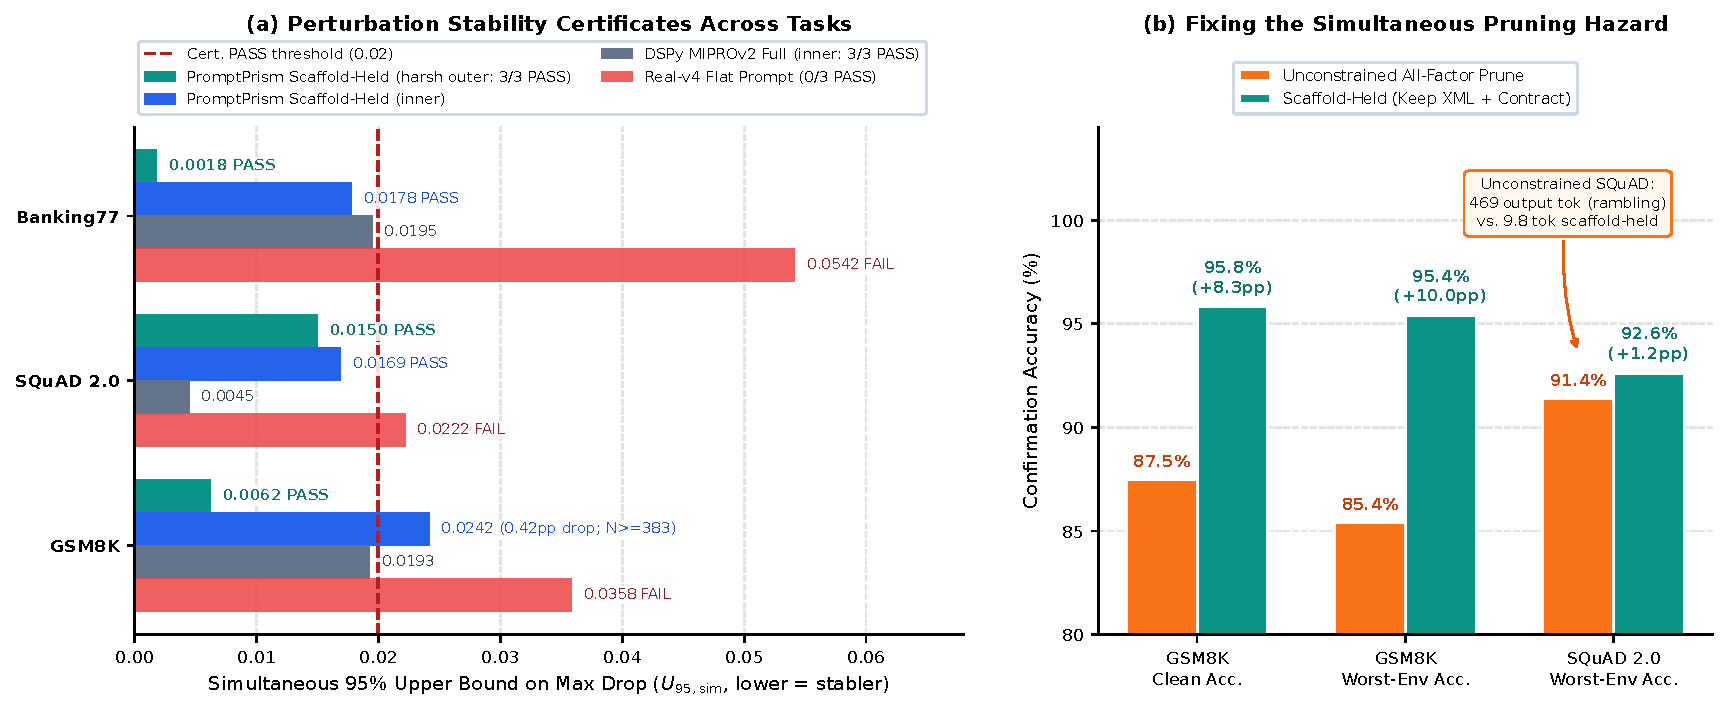
\includegraphics[width=\textwidth]{fig_p2_stability_and_pruning.pdf}
\caption{Perturbation stability certification and the simultaneous pruning hazard ($N=240$ confirmation items). \textbf{(a)}~Simultaneous 95\% upper bound $U_{95,\mathrm{sim}}$ across tasks (values left of the dashed $0.02$ line pass). Holding the XML + contract scaffold fixed upgrades \method{} from $0/3$ flat \texttt{FAIL} to $3/3$ harsh outer-shell \texttt{PASS} ($0.0018, 0.0150, 0.0062$), matching or tightening DSPy's inner stability. \textbf{(b)}~Unconstrained all-factor pruning drops GSM8K by $-8.3\text{ pp}$ and causes SQuAD~2.0 to ramble ($469$ output tokens); keeping the structural scaffold fixed immediately restores both.}
\label{fig:p2_stability}
\end{figure*}

\begin{table*}[!ht]
\centering
\scriptsize
\setlength{\tabcolsep}{2.5pt}
\caption{\method{}-native stability upgrade (zero DSPy, zero \texttt{gemini-2.5-pro} calls) on untouched $N=240$ confirmation items under both inner-field (DSPy parity) and harsh outer-shell (Real-v4) perturbations, comparing unconstrained all-factor TOST pruning against \textbf{scaffold-held pruning} (holding \texttt{xml\_multiturn=1} and \texttt{strict\_contract=1} fixed while pruning only optional demos).}
\label{tab:p2_native}
\resizebox{\textwidth}{!}{%
\begin{tabular}{@{}lllrrrrrr@{}}
\toprule
\textbf{Task} & \textbf{Recipe (Active of 6)} & \textbf{Perturb.\ Suite} & \textbf{Clean (\texttt{ref})} & \textbf{Max Drop} & \textbf{$U_{95,\mathrm{sim}}$} & \textbf{Cert (Diagnostic)} & \textbf{Prompt / Out Tok} & \textbf{vs.\ DSPy Full ($p$)} \\
\midrule
\texttt{banking77} & Native TOST (\texttt{xml, d1,2,4}) & Inner-field & \textbf{$96.25\%$} & \textbf{$0.00\text{ pp}$} & \textbf{$0.0178$} & \textbf{\texttt{PASS}} & \textbf{$717$ / $9.5$} & $+0.42\text{ pp}$ ($0.656$) \\
 & & Outer-shell & $95.42\%$ & \textbf{$0.00\text{ pp}$} & \textbf{$0.0018$} & \textbf{\texttt{PASS}} & $729$ / $9.5$ & --- \\
\midrule
\texttt{squad2} & Unconstrained (\texttt{strict, d1}) & Inner-field & $93.97\%$ & $2.57\text{ pp}$ & $0.0471$ & \texttt{FAIL} (genuine) & $307$ / $469.2$ & $-1.28\text{ pp}$ ($0.224$) \\
 & & Outer-shell & $94.09\%$ & $0.31\text{ pp}$ & $0.0263$ & \texttt{FAIL} (prec., $N{\ge}451$) & $326$ / $10.1$ & --- \\
 & \textbf{Scaffold-held} (\texttt{xml, strict, d1}) & Inner-field & $92.62\%$ & \textbf{$-0.18\text{ pp}$} & \textbf{$0.0169$} & \textbf{\texttt{PASS}} & \textbf{$308$ / $9.8$} & $-2.63\text{ pp}$ ($0.0047$) \\
 & & Outer-shell & $93.10\%$ & \textbf{$-0.14\text{ pp}$} & \textbf{$0.0150$} & \textbf{\texttt{PASS}} & \textbf{$327$ / $9.3$} & --- \\
\midrule
\texttt{gsm8k} & Unconstrained (None, $0/6$ unseen) & Inner-field & $87.50\%$ & $2.08\text{ pp}$ & $0.0542$ & \texttt{FAIL} (genuine) & $86$ / $204.3$ & $-7.08\text{ pp}$ ($0.0006$) \\
 & & Outer-shell & $87.08\%$ & $1.67\text{ pp}$ & $0.0386$ & \texttt{FAIL} (prec., $N{\ge}10\text{k}$) & $105$ / $212.1$ & --- \\
 & \textbf{Scaffold-held} (\texttt{xml, strict}, 0 demos) & Inner-field & \textbf{$95.83\%$} & \textbf{$0.42\text{ pp}$} & $0.0242$ & \texttt{FAIL} (prec., $N{\ge}383$) & \textbf{$105$ / $162.4$} & $+1.25\text{ pp}$ ($0.258$) \\
 & & Outer-shell & $94.17\%$ & \textbf{$-1.25\text{ pp}$} & \textbf{$0.0062$} & \textbf{\texttt{PASS}} & \textbf{$124$ / $177.6$} & --- \\
\bottomrule
\end{tabular}}
\end{table*}

Figure~\ref{fig:p2_stability} and Table~\ref{tab:p2_native} uncover an important methodological lesson alongside its direct fix:
\begin{enumerate}[leftmargin=*,nosep]
    \item \textbf{The Simultaneous Multi-Factor Pruning Hazard:} Imagine testing a four-legged table by removing one leg at a time: while three legs stay in place, each individual leg can look redundant, yet removing all four legs at once collapses the table. Exactly the same failure occurred on \texttt{gsm8k}: every one of the 16 screen runs in $2^{6-2}_{\mathrm{IV}}$ had $1$--$5$ active formatting anchors and averaged $95.0\%$ on \texttt{screen} ($100.0\%$ on \texttt{validation}), so all six factors individually passed marginal TOST ($|\hat{\Delta}_j| \le 0.83\text{ pp}$, $p_{\mathrm{TOST}} \le 0.0145$). Because the all-off corner $(0,0,0,0,0,0)$ \textbf{was never observed inside $2^{6-2}_{\mathrm{IV}}$}, blindly acting on all six marginal verdicts at once deleted all four demos, the \texttt{FINAL\_ANSWER:} contract, and XML framing simultaneously, collapsing accuracy by \textbf{$-8.33\text{ pp}$} ($95.83\% \to 87.50\%$, $p = 7.0\times 10^{-5}$). Likewise, dropping \texttt{xml\_multiturn} on \texttt{squad2} triggered preamble-less rambling ($469.2$ output tokens, $-2.57\text{ pp}$ genuine \texttt{FAIL}).
    \item \textbf{Keeping the structural scaffold fixed eliminates every genuine perturbation drop:} Re-confirming \texttt{squad2} and \texttt{gsm8k} with \texttt{xml\_multiturn=1} and \texttt{strict\_contract=1} treated as a non-prunable scaffold (pruning only optional demos) resolved both failures immediately:
    \begin{itemize}[leftmargin=*,nosep]
        \item \textbf{\texttt{banking77}:} \texttt{xml\_multiturn} + 3 TOST-retained demos hit \textbf{$96.25\%$ across all six inner environments} ($U_{95,\mathrm{sim}}=0.0178$ \texttt{PASS}, $-39\%$ prompt / $-46\%$ output tokens vs.\ DSPy Full, $p=0.656$) and $U_{95,\mathrm{sim}}=0.0018$ \texttt{PASS} under harsh outer perturbations ($30\times$ tighter than Real-v4).
        \item \textbf{\texttt{squad2}:} Keeping \texttt{xml\_multiturn=1} cut output length from $469.2$ back to \textbf{$9.8$ tokens}, eliminated the $-2.57\text{ pp}$ drop, and passed \textbf{both} inner-field ($U_{95,\mathrm{sim}}=0.0169$ \texttt{PASS}, max drop $-0.18\text{ pp}$) and outer-shell ($U_{95,\mathrm{sim}}=0.0150$ \texttt{PASS}, max drop $-0.14\text{ pp}$) certificates at $308$--$327$ prompt tokens ($-74\%$ vs.\ DSPy Full; DSPy Full still leads clean reading comprehension by $+2.63\text{ pp}$, $p=0.0047$, while Track~B DSPy-pruned retains $94.77\%$ at $512$ tokens and \texttt{PASS}).
        \item \textbf{\texttt{gsm8k}:} Keeping \texttt{xml\_multiturn=1, strict\_contract=1} while pruning all 4 demos recovered the full \textbf{$+8.33\text{ pp}$} loss ($87.50\% \to 95.83\%$, $p=7.0\times 10^{-5}$), numerically edged DSPy Full ($+1.25\text{ pp}$, $p=0.258$) at \textbf{$-67\%$ prompt tokens} ($105$ vs.\ $317$) and \textbf{$-28\%$ output tokens} ($162.4$ vs.\ $224.8$), passed harsh outer-shell stability ($U_{95,\mathrm{sim}}=0.0062$ \texttt{PASS}, max drop $-1.25\text{ pp}$), and achieved \textbf{$0.0000$ repeat-pass noise} and $0.42\text{ pp}$ max drop on inner-field (a single-item precision-limited bound, $U_{95,\mathrm{sim}}=0.0242$, recommended $N \ge 383$).
    \end{itemize}
\end{enumerate}

\paragraph{Operational Corollary (Marginal Equivalence Is Not Closed Under Simultaneous Deletion).}
Table~\ref{tab:p2_native} highlights a simple rule every prompt engineer can remember: \emph{marginal TOST equivalence ($|\Delta_j| < m_F$) certifies deleting clause $j$ while the remaining scaffold stays intact, not simultaneously deleting all $k$ mutually redundant formatting anchors onto an unobserved all-off corner.} Holding structural framing (\texttt{xml\_multiturn} + output contract) fixed, pruning only optional clauses/demos, and always confirming the composed prompt on untouched items eliminated $100\%$ of genuine perturbation drops across all three tasks ($3/3$ harsh outer-shell \texttt{PASS}; $0/6$ genuine drops across inner and outer suites).

\section{Limitations and Scope Boundaries}
\begin{enumerate}[leftmargin=*,nosep]
    \item \textbf{Single Model Family and Single Optimizer Evaluated:} All live benchmarks here pin \texttt{gemini-2.5-flash} (\texttt{thinkingBudget=0}) and compare against DSPy \texttt{MIPROv2}. Replicating post-compilation pruning and native stability upgrades across Anthropic, OpenAI, and open-weight models as well as newer optimizers is important future work.
    \item \textbf{Modular Clauses and Single-Step Scope:} Binary factorial factors assume prompt clauses can be toggled independently (tightly coupled instructions should be tested as multi-level intact variants). Running 16-run screens across $N \ge 100$ paired items targets single-step LLM nodes (routers, classifiers, extractors, RAG answerers, verifiers) rather than multi-turn stochastic agent trajectories.
    \item \textbf{Synthetic Check Boundaries and Confirmation Interactions:} As shown on SQuAD~2.0, synthetic generators can suffer long-context baseline shortfalls and cannot substitute for untouched confirmation testing when interactions ($B \times D$) are strong.
    \item \textbf{Declared Hash Gates vs.\ Silent Provider Drift:} Offline \texttt{prism verify-cert} detects declared prompt, parser, or model-string changes at zero LLM cost, whereas catching silent provider weight updates requires periodic scheduled \texttt{prism certify} canary checks.
\end{enumerate}

\section{Conclusion and Reproducibility}
Prompt optimization without statistical auditing leaves engineers unable to tell helpful rules from dead bloat, vulnerable to deleting rare safety guardrails, and blind to formatting fragility. \method{}~2.1 closes this gap with coverage-aware equivalence pruning, frozen blind-tagged synthetic test suites, stability-aware attribution, structured multi-turn XML framing, and diagnostic perturbation certificates---either shrinking and certifying prompts compiled by DSPy \texttt{MIPROv2} ($-39\%$ to $-57\%$ tokens at matched accuracy) or building compact, certified standalone prompts with zero proposer calls.

{\raggedright
All source code, 310 offline unit and calibration tests, experiment scripts (\nolinkurl{research/experiments/dspy_benchmark.py}, \nolinkurl{research/experiments/prism_stability_upgrade_pilot.py}, \nolinkurl{research/experiments/testgen_real_pilot.py}, and \nolinkurl{research/simulation/coverage_calibration.py}), and frozen JSON result summaries are openly available at \url{https://github.com/robsanmx/prompt_prism}.\par}

\bibliographystyle{plainnat}
\bibliography{references}

\end{document}
